\label{annex:fmcw-radar-processing}
% The operating principles of the sensors, and applicable signal processing algorithms,
% are discussed in the second chapter of the thesis.

% Theory (24)
The sensor assembly consists of four devices:
an \gls{fmcw} radar, an \gls{ir} camera, an RGB-D camera, and a 16-channel microphone.
With these sensors, the location, posture, and emitted sound of a person can be observed.
The radar offers a range-azimuth location and a Doppler-spectrum. % TODO: Cite
The \gls{ir} and RGB-D cameras excel at posture estimation,  % TODO: Cite
but can also be used for range and azimuth estimation; especially the depth camera. % TODO: Cite
The microphone simply records the sound, 
but it may also be used to estimate the \gls{aoa} of the recorded sounds. % TODO: Cite
Different sounds can also be used as additional data for activity recognition. % TODO: Cite

The operating principles of the sensors will be briefly discussed in the upcoming sections.
The \gls{ir} and RGB-D cameras used for the system have on-board data processing and 
output images than can be used in learning algorithms without further processing. % TODO: cite
Their signal processing is therefore out of scope for this thesis.
The microphone simply outputs an I/Q sampled audio signal on all channels.
The signal processing is very elementary and will not be discussed,
except for the case of \gls{aoa} estimation i.e. beam forming.

The radar device used for the system has capabilities for on-board signal processing 
and can output data that could be used as-is for learning algorithms,
but simply reading the raw radar samples
and processing them after recording unlocked much greater performance.
Along the operating principles,
the used signal processing and target detection algorithms will be discussed.

%% Sensors
\section{Radar}
%% Radar
%%% How radars are categorised
%       - Pulse/CW, Monostatic/Bistatic
%%% Radar processing algorithms
%       - What kind of radar we are using
%       - Fourier algos
%       - Music algos
%       - Target detection
%       - Target tracking

% TODO: The chosen radar is capable of all operating modes but was used in the fmcw mode
% The operating principles for all the CW type radars will be briefly discussed,
% but more detailed signal processing will only be discussed for the FMCW radar.

Radars can be categorized based on their emitted wave form into two principal categories:
the pulse radar, and the contiuous-wave radar.
Furthermore, radars can also be categorized 
based on the relative location of the transmitter and receiver
into monostatic and bistatic radars.
This section will begin with a brief overview of the different categories of radar,
followed by a deeper dive into signal processing of the radar used for the sensor assembly.

The pulse radar, as the name suggests, emits pulses of energy.
These pulses can be of very high energy,
which allows it to reach ranges even further than the horizon. % Cite: OTH Radar
Additionally, the signal processing is fairly simple.
Range can be calculated simply from the time elapsed between emitting and receiving the pulse,
and velocity can be calculated by applying a Fourier transform to the received signal,
and calculating the Doppler shift.
The waveform of a pulse radar is illustrated in Figure \ref{fig:pulse_waveform}.

\begin{figure}
    \centering
    
\includegraphics[width=\textwidth]{fig/placeholder.png}
    \caption{Waveform of the pulse radar.}
    \label{fig:pulse_waveform}
\end{figure}

While the massive range can be useful in some applications,
the pulse radar also suffers from a very high peak-to-average power ratio.
This translates into expensive components and therefore high cost.

Due to the high cost,
the continuous-wave radar is often a better choice for short range applications.
The continuous-wave radar, as the name again suggests,
does not emit pulses, but instead a continuous wave.
The continuous-wave radar can be further divided into three subcategories 
based on the emitted waveform:
\gls{cw}, \gls{fmcw}, and \gls{fsk}.
The different continuous-wave radar subcategories are defined by their emitted wave form,
illustrated in Figure \ref{fig:cw_waveforms}.

\begin{figure}[H]
    \centering
    \begin{subfigure}[b]{\textwidth}
        \centering
        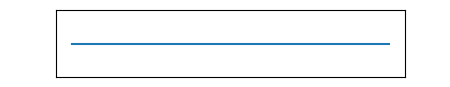
\includegraphics[width=\textwidth]{fig/2/cw_wave.png}
        \caption{\gls{cw} radar.}
        \label{fig:cw}
    \end{subfigure}

    \begin{subfigure}[b]{\textwidth}
        \centering
        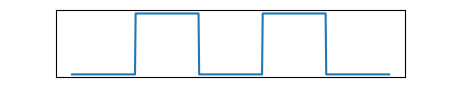
\includegraphics[width=\textwidth]{fig/2/fsk_wave.png}
        \caption{\gls{fsk} radar.}
        \label{fig:fsk}
    \end{subfigure}

    \begin{subfigure}[b]{\textwidth}
        \centering
        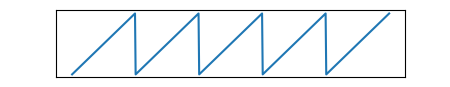
\includegraphics[width=\textwidth]{fig/2/fmcw_wave.png}
        \caption{\gls{fmcw} radar.}
        \label{fig:fmcw}
    \end{subfigure}

    \caption{Different types of constant waveform signals.
                Frequency on y-axis and time on x-axis.}
    \label{fig:cw_waveforms}
\end{figure}

The \gls{cw} radar (Figure \ref{fig:cw}) is the simplest of the three.
As the figure shows, it is simply a constant tone.
With simple design, also comes simple signal processing.
Finding the velocity of a target is a simple matter of figuring out the Doppler-shift
of the received signal.
Sadly, though, the \gls{cw} radar is unable to detect the range of a target.

Since the range of a target is determined based on the round-trip-time of the signal,
the signal needs to be time variant.
While the \gls{cw} radar is technically time variant,
the period of the signal is too short for a meaningful maximum unambiguous range.
By varying the emitted frequency over time,
the period of the signal can be elongated significantly,
which allows for determining the range of a target.
Both the \gls{fmcw} and \gls{fsk} radar achieve this with slightly different approaches.

In the \gls{fsk} radar,
the frequency of the signal is periodically shifted between two or more frequencies,
as shown in Figure \ref{fig:fsk}.
The velocity of a target is still calculated from the Doppler-shift,
but the range is calculated based on the length of the square pulse
that remains after downconversion of the received signal,
as illustrated in figure \ref{fig:fsk_range}.

\begin{figure}
    \centering
    
\includegraphics[width=\textwidth]{fig/placeholder.png}
    \caption{With \gls{fsk} radar, 
        the range is calculated from the phase difference of the square waves.}
    \label{fig:fsk_range}
\end{figure}

Longer pulses translate into a higher maximum unambiguous range
with the cost of a lower frame rate.
Shorter pulses can be used to achieve a higher frame rate 
at the cost of lower maximum unambiguous range.
With shorter range, 
a problem arises where an echo from a previous step could be received
while the next one is already being transmitted.
This can be counteracted via using multiple frequency steps and filtering.
Although this method can achieve long maximum unambiguous ranges with a relatively small bandwidth,
this method of measuring the length of the resulting square signal is computationally complex
and has a higher latency than what could be achieved with the \gls{fmcw} radar.

The \gls{fmcw} radar resembles an \gls{fsk} radar,
but the number of frequency steps approaches infinite.
Consequentially, the waveform becomes a triangle or a sawtooth wave,
as seen in Figure \ref{fig:fmcw}.

With the \gls{fmcw} radar,
calculating the range of a target is computationally easier than with the \gls{fsk} radar.
The signal frequency changes linearly in time,
meaning the signal round-trip-time can be calculated from the frequency difference
between the emitted signal and received echo.
The Fourier transform, therefore, tells the range of a target.

The velocity of a target can also be determined via the Fourier transform.
When the target is detected multiple times in a very short time,
it will be detected in the same range bin,
but due to the very small change in distance,
the received echo will be in a different phase.
The velocity can then be determined 
by taking the Fourier transform across these multiple range measurements.
This is further explained in Section \ref{sec:processing}.

The \gls{fmcw} radar can also reach high maximum unambiguous ranges
by using waveforms with a long ramp in the time domain.
Sadly, though, the range resolution is severely limited 
as it is proportional to the bandwidth of the signal:
$d_{res} = c/2B$, where $d_{res}$ is the range resolution and $B$ is the signal bandwidth.
While on low frequencies the range resolution is very poor,
on millimetre-wave bands the bandwidths can be increased substantially 
and the range resolution can be reduced to only a few centimetres.

% Monostatic and bistatic
As stated earlier,
radars can also be categorized into monostatic and bistatic radars
based on the receiver configuration.
In the monostatic radar,
the transmitter and receiver are located in the same place,
whereas in the bistatic radar the receiver is located in a different place than the transmitter.
This is demonstrated in Figure \ref{fig:monostatic_bistatic}.

\begin{figure}
    \centering
    
\includegraphics[width=\textwidth]{fig/placeholder.png}
    \caption{Monostatic and bistatic radar.}
    \label{fig:monostatic_bistatic}
\end{figure}

Both receiver configurations have their advantages and disadvantages.
With the bistatic radar, the receiver can be made relatively light and mobile.
It can also exploit a third-party radio signal.
This can be used for radar detection or passive radar, among other uses.
As a downside, the system design and signal processing is more complex 
as the range between the transmitter and target is different from the range between the receiver and the target.
Furthermore, if when a third-party signal is used, it may not be known exactly.

The monostatic radar, on the other hand,
has a simpler system design as the transmitted signal is always known, 
and the received signal can be converted onto baseband frequency simply 
by mixing the transmitted and received signals.
As a downside, the transmitter and receiver are tied to the same location.
When the transmitter is immobile,
a bistatic configuration may be able to achieve better signal-to-noise ratio in the receiver
as the receiver can potentially be brought closer to the target.
In some applications, there may also be multiple parties who need to do radar detection,
but it may be unfeasible to power a transmitter,
or it may simply be cheaper to have one powerful transmitter and multiple simple receivers.
In many cases, though,
the monostatic configuration is the better choice due to sheer simplicity.

The radar used in the sensor assembly is of the monostatic type,
operates on 60--64 GHz frequency,
and is capable of all continuous-wave operating modes.
In this project, it was used in the \gls{fmcw} mode with a sawtooth wave,
see Figure \ref{fig:fmcw}.

In the next section (\ref{sec:processing}),
the radar processing algorithms are presented,
that are applicable of the \gls{fmcw} radar and were used in this project.

\section{FMCW Radar processing}
\label{sec:processing}
% Sampling and data cube
% Waveform overview
%   - what measurement tells what
% FFT and Correlation approaches
%   - pros and cons of each
The radar used for the assembly is a continuous-wave monostatic radar.
The block diagram of the transceiver is shown in Figure \ref{fig:rxtx_block_diagram}.
\begin{figure}
    \centering
    
\includegraphics[width=\textwidth]{fig/placeholder.png}
    \caption{Transmitter and receiver block diagram.}
    \label{fig:rxtx_block_diag}
\end{figure}
The monostatic continuous-wave radar has two antennas.
One of them emits the signal $s_{tx}(t)$ and the other one receives the echoes $s_{e}(t)$.
Due to self-interference, the signal heard by the receiver is actually a combination of both: 
$s_{rx}(t) = s_{tx}(t)s_{e}(t)$.
The echoes can be isolated from $s_{rx}(t)$ by mixing it with $s_{tx}(t)$
and applying a low-pass filter: $s_{e}(t) = s_{tx}(t)s_{rx}(t)$.
This is based on the trigonometric identity
\begin{equation}
    \label{eq:trig}
    \sin (2 \pi f_1 t) \sin (2 \pi f_2 t) 
    = \frac{1}{2} \cos [2 \pi ( f_1 - f_2 )t] - \frac{1}{2} \cos [2 \pi ( f_1 + f_2 ) t].
\end{equation}

This also has the property of converting $s_{e}(t)$ into a baseband signal,
as shown in Figure \ref{fig:fmcw_mixing}.
The remaining non-zero frequencies are called beat frequencies
 and are caused by the received echoes.
The beat frequencies can be used to find the range of a target.

\begin{figure}
    \centering
    
\includegraphics[width=\textwidth]{fig/placeholder.png}
    \caption{Above are the transmitted signal (blue) and received signal (red).
        Below is the resulting baseband signal after mixing.}
    \label{fig:fmcw_mixing}
\end{figure}

The transmitted signal $s_{tx}(t)$ consists of multiple chirps.
A chirp is simply a signal that rises in frequency linearly.
Figure \ref{fig:fmcw_waveform_annotated} shows $s_{tx}(s)$ above and $s_{e}(s)$ below.
The parts of the signal are annotated in the figure along the sampling periods.

\begin{figure}
    \centering
    
\includegraphics[width=\textwidth]{fig/placeholder.png}
    \caption{Sampling periods annotated along emitted signal and received echoes.}
    \label{fig:fmcw_waveform_annotated}
\end{figure}

As figure \ref{fig:fmcw_waveform_annotated} shows,
each chirp is sampled $N$ times, and the chirps are repeated $M$ times.
The $N$ samples of a single chirp are called fast-time samples
and the $M$ chunks of fast-time samples are called slow-time samples.
These can be arranged in a matrix format, as shown in Figure \ref{fig:radar_matrix}.

\begin{figure}
    \centering
    
\includegraphics[width=\textwidth]{fig/placeholder.png}
    \caption{Radar data matrix.}
    \label{fig:radar_matrix}
\end{figure}

When multiple ($K$) antennas are used in the receiver,
the same sampling can be performed for multiple antennas,
and the phase of the received signal will be slightly different in each antenna
based on the \gls{aoa}.
The samples taken from different receiver antennas are called spatial samples.
The $K$ spatial samples create a third dimension in the radar data matrix,
thus creating a radar data cube (Figure \ref{fig:radar_cube}).

\begin{figure}
    \centering
    
\includegraphics[width=\textwidth]{fig/placeholder.png}
    \caption{Radar data cube.}
    \label{fig:radar_cube}
\end{figure}

The different dimensions of the radar data cube give different information.
The fast time samples give range information,
the slow-time samples five velocity information,
and the spatial samples give angular information.
There are two principal ways of getting this information from the data cube.

The Fourier transform is a computationally efficient method of getting the range and velocity information.
It can also be used for angular information,
but as there are only $K$ samples, 
there are only $K-1$ angle bins after the discrete Fourier transform.
The number of angle bins is therefore limited by the number of antennas.

Correlation is a computationally much heavier approach,
but it can achieve an arbitrary number of angle bins.
The same applies for range and velocity,
but the Fourier transform approach results in an adequate number of bins for both,
meaning the correlation approach is the most useful for angular information.
In the correlation approach, instead of limiting the number of angle bins,
the number of antennas limits the angular resolution,
i.e. the minimum angle where two targets can be distinguished.

Next, data processing algorithms will be presented for both approaches.
Following that, target detection and tracking will be discussed.

\subsection{Determining the range and angle}
\label{sec:range_angle}
The \gls{fmcw} radar emits chirps with a slope ($S$) that rise in frequency over time ($S$ Hz/s),
which makes it easy to measure the round-trip time of the signal.
At each moment, a certain frequency is emitted.
The signal with this frequency then echoes off a target and is received $t$ seconds later.
At this moment, another frequency is being emitted.
The signals are then mixed, giving a beat frequency $f_b$.
This gives a fully defined triangle from which the round-trip $t_{rt}$ time can be calculated.
This is illustrated in Figure \ref{fig:fmcw_triangle}.
\begin{figure}
    \centering
    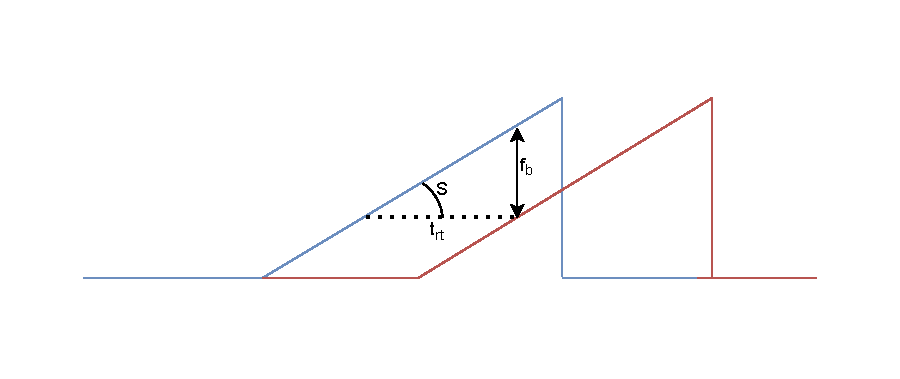
\includegraphics[width=.9\textwidth]{fig/2/fmcw_triangle.pdf}
    \caption{The relationship between slope, beat frequency, and round-trip time.
    The emitted signal is blue and received signal is red.}
    \label{fig:fmcw_triangle}
\end{figure}
In mathematical form, the relationship between the slope, beat frequency, and round-trip time is
$f_b = S t_{rt}$ or $t_{rt} = \frac{f_b}{S}$.
The distance the signal travels is therefore $t_{rt}c$,
and the range of the target is half of that.
The range of the target ($R(\cdot)$) as a function of $f_b$ is therefore
\begin{equation}
    \label{fmcw_range}
    R \left ( f_{b} \right ) = \frac{f_{b}c}{2S}.
\end{equation}

% TODO
One way of determining the beat frequency
is applying the Fourier transform to the fast-time samples.
\begin{itemize}
    \item Range resolution
    \item Maximum unambiguous range
    \item likely 3-4 paragraphs
\end{itemize}

The Fourier transform could technically be applied to the spatial samples
to determine the \gls{aoa}.
The angular resolution would in this case be $FOV / K-1$.
% TODO: check math
The number of receiver antennas is often fairly low, though,
resulting in abysmal angular resolution.

Another way to determine the range and angle of a target is by using correlation.
This is called the \gls{music} algorithm.
It can be applied separately to fast-time or spatial samples,
or both can be combined to the same algorithm.
In the latter case, it is called the 2D-\gls{music} algorithm.

% TODO
\begin{itemize}
    \item Range-music
    \item Angle-music
    \item 1D Spatial smoothing
    \item 2D-MUSIC
    \item 2D Spatial smoothing
    \item likely 7-12 paragraphs
\end{itemize}

\subsection{Determining the velocity}
\label{sec:velocity}
The velocity of the target is determined based on the slow-time samples.
When the same target is detected multiple times in a short time,
the phase of the echo changes slightly.
This shift in phase depends on how much the target moved between the slow-time samples,
as illustrated in Figure \ref{fig:fmcw_slow_time_principle}.
\begin{figure}
    \centering
    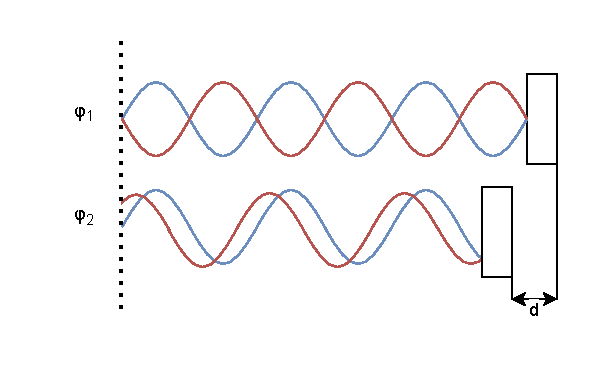
\includegraphics[width=.9\textwidth]{fig/2/fmcw_slow_time_principle.pdf}
    \caption{The phase-shift between slow-time samples depends on the distance moved by the target.}
    \label{fig:fmcw_slow_time_principle}
\end{figure}

%The phase-shift between each slow-time sample depends on multiple variables:
%the signal wavelength, target velocity, and sampling frequency.
%It can be formulated as $\phi = 2 \pi (d / \lambda)$, 
%where $\phi$ is the phase-shift, $d$ is the moved distance, and $\lambda$ is the wavelength.
%The target moves $v T_c$ meters per sample, 
%where $v$ is the velocity and $T_c$ is the sampling period.

The consecutive phase-shifts create an oscillation,
whose frequency can be determined again with either the Fourier transform or correlation.
The relationship between velocity and the slow-time frequency is
\begin{equation}
    v = \frac{c f}{2 f_c},
\end{equation}
where $f_c$ is the frequency of the transmitted signal
and $f$ is the frequency observed in the slow-time samples.

The maximum unambiguous velocity is such a velocity,
where the target moves less than half a wavelength between each slow-time sample.
This is in accordance to the Nyquist theorem:
% TODO: Cite
if a wave is sampled less than twice per oscillation, there will be aliasing.
The sampling frequency is $T_{c}^{-1}$, 
which is twice the maximum unambiguous frequency in the slow-time samples.
Thus results a maximum unambiguous velocity of
\begin{equation}
    v_{max} = \frac{c T_{c}^{-1}}{4 f_c} = \frac{\lambda}{4 T_c}.
\end{equation}

Again, with the correlation method an arbitrary velocity resolution can be achieved.
With the Fourier transform, though,
the resolution depends on the number of slow-time samples and the maximum unambiguous velocity.
Since a single chirp produces a single slow-time sample,
the number of slow-time samples is determined by how many chirps are included in a single frame.
With $M$ slow-time samples, $M-1$ velocity bins can be observed after the Fourier-transform.
The resulting velocity resolution is therefore
\begin{equation}
    \Delta v = \frac{v_{max}}{M-1}
\end{equation}

\subsection{Target detection and tracking}
\label{sec:target}
% Detection basics
%   - false alarm rate with constant threshold
% CFAR as the superior option

\section{RGB-D camera}
% Depth camera operating principle
% Pixel as a measurement of angle
% Pixels as a measurement of distance
In addition to the typical RGB video,
the RGB-D camera records a stereo video using two cameras separated by a small distance.
Using similar principles as human vision,
depth information can be extracted from this stereo video.
% TODO: Explain further or reference an explanation
Furthermore, the depth information can be improved
for example via the use of an uniform infrared dot matrix.

The point of origin for each \gls{ir} beam is the same,
and the angular separation is known.
Thus, distance from the camera is directly proportional to the distance
separating the projected dots.
% TODO: citation; maybe this 
This is illustrated in figure \ref{fig:ir-dot-matrix}

\begin{figure}
    \centering
    
\includegraphics[width=\textwidth]{tex/fig/placeholder.png}
    \caption{Relationship between inter-dot distance and camera-to-dot distance.}
    \label{fig:ir-dot-matrix}
\end{figure}

In addition to the depth-channel,
also the RGB-channel can be used for depth measurement in a limited fashion.
Given a camera with \gls{fov} of $N$ by $M$ degrees
and a resolution of $n$ by $m$,
each pixel has an individual \gls{fov} of $N/n$ degrees in the first dimension,
and $M/m$ degrees in the second dimension.

Similar to the \gls{ir} dot matrix,
the width (in units of distance) of each pixel is directly proportional
to the distance from the camera.
By placing solid-colour squares with known dimensions on different distances
in the vision of the camera,
the number of pixels a square encompasses 
can be used to calculate the distance from the camera.

The main attraction of the camera in the context of \gls{har}
is posture estimation.
Certain postures, or chains of postures,
correlate very well with specific actions.
For example, a sitting posture followed by a standing posture 
very likely means that a person stood up.

Additionally, object detection can also be used to infer the target of the action,
and face recognition can be used to detect who performed the action.

Although the information listed heretofore can be gathered
from the RGB video alone,
some qualities can be improved with the depth video.
Specifically, the depth-channel can be used to improve object separation
in the data processing,
which in turn can be used to improve object detection,
and moreover posture estimation.
% TODO: Cite

\section{Infrared camera}
% Role of IR in the assembly
%   - what IR does better than RGB (low-visibility: too dark, foggy, or too bright, or low contrast)
%   - How IR can supplement radar detection
A low-resolution infrared camera could be considered both
an auxillary sensor for the whole assembly,
and an alternative option to the RGB camera.

Although the resolution of the \gls{ir} camera used in the assembly
is awfully low,
human figures and certain postures can still be detected with reasonable accuracy
from the video stream, at least with the bare eye and using interpolation
to improve the resolution.
Also, given a larger budget, the resolution of the \gls{ir} camera could be increased.

The \gls{ir} camera could possibly be used in place of the RGB camera
in conditions where the RGB camera is not likely to work,
such as dark, foggy, overwhelmingly bright, or low contrast.
This applies to many outdoor environments:
\begin{itemize}
    \item at night time there may not be enough light,
    \item sometimes thick fog can reduce visibility,
    \item in direct sunlight the RGB camera sensor may become overloaded,
    \item and in certain environments the colour contrast is very little but thermal contrast is very high.
\end{itemize}

Furthermore, the data from the \gls{ir} video 
can be used to detect targets of interest.
This could lead to improved clutter detection in the radar,
or simply sensor assembly power savings as some sensors may be turned off
while waiting for targets of interest.


\section{16-channel microphone and beam forming}
% How sound can be used in HAR
% beam forming as as means of antenna direction
In terms of \gls{har},
a microphone provides information about which activities are performed.
Certain activities produce certain noises, 
e.g. eating, writing on a computer keyboard, flipping pages.
If the sound signatures of activities can be detected,
the information can be used to increase the activity detection accuracy.

In addition,
when there are multiple detected activities 
that look similar to the other sensors,
if the sound \gls{aoa} could be detected,
it could be determined which target is emitting which sound,
and thus the activities could be detected with higher accuracy in this situation.

For \gls{aoa} detection,
a uniform linear array of microphones is a simple solution.
The principle is exactly the same as in the case of electromagnetic waves.
% TODO: reference
The echoing and overall structure of sound signals is much more complex than
of electromagnetic signals, though.
% TODO: research solutions and write a few sentences

%%%%%%%%%%%%%%%%%%%%%%%%%%%%%%%%%%%%%%%%%%%%%%%%%%%%%%%%%%%%%%%

%\section{Human Activity Recognition and Machine Learning}
% Posture estimation
%% Video streams (IR, RGB, Depth)
% Sound detection
% Micro-doppler

%\section{Sound angle-of-arrival detection}

%%%%%%%%%%%%%%%%%%%%%%%%%%%%%%%%%%%%%%%%%%%%%%%%%%%%%%%%%%%%%%%
%\section{Dataset requirements}